\chapter{Фазовая диаграмма}\label{ch:ch3}

\section{Теоретическая магнитная фазовая диаграмма в отсутствии поля} Каждый образец содержал долю $P_{+}$ ферромагнитных связей  $J_{ij}=+1$. Все взаимодействия были только антиферромагнитными $J_{ij}=-1$, если $P_{+}=0$. Для каждой концентрации $P_{+}$ было получено по десять образцов со случайным равномерным распределением $J_{ij}$. 

Границы фаз или критические температуры переходов ''ферромагнетизм-спиновое стекло''  и ''антиферромагнетизм-спиновое стекло'' $T(P_{+})$ получены приближенно, как температуры точек перегиба параметра фрустраций \cite{makarov2019} 

\begin{equation}
	F_p(T) = \frac{E_{max} + \langle E \rangle (T)}{2E_{max}},
	\label{eq:frustration_parameter}
\end{equation}
см. рисунок \ref{fig:fp0}. 

\begin{figure}[!ht]
	\centering
	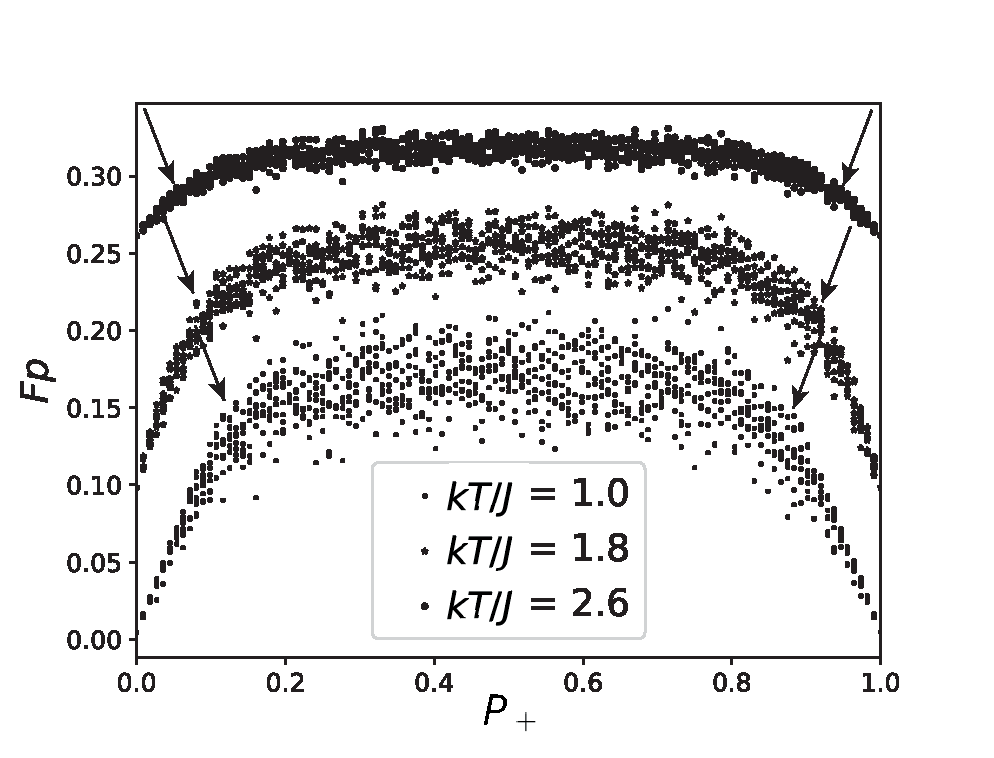
\includegraphics[width=0.7\linewidth]{Frustration_parameter_h0.0.eps}
	\caption{Зависимость параметра фрустрации от концентрации $P_{+}$ обменных констант для образцов $N=8\times8$ без внешнего поля для температур, указанных на вставке}
	\label{fig:fp0}
\end{figure}

Максимальная энергия системы $E_{max}$ --- сумма по модулю всех парных энергий взаимодействия. В отличном от нуля поле энергия Зеемана добавляется в виде слагаемого с максимальным спиновым избытком

\begin{equation}
	E_{max} = 2NJ_{ij}(N-1) + MH, \quad M = N.
	\label{eq:Emax}
\end{equation}

Граница фаз ''парамагнетик-спиновое стекло'' определена путем численных расчетов температуры максимума теплоемкости $C_{max}(T)$ в температурной зависимости
\begin{equation}
	C(T)=\frac{\partial \langle E \rangle (T)}{\partial T}=\frac{\langle E^2 \rangle-\langle E \rangle ^2}{k T^2},
	\label{eq:ct}
\end{equation}
где
\begin{equation}
	\langle E \rangle (T) =\frac{1}{Z}\sum_{t=1}^{\Omega}g_t E_t \exp\left\{-\frac{E_t}{kT}\right\}
	\label{eq:ct}
\end{equation}
и
\begin{equation}
	\langle E^2 \rangle (T) =\frac{1}{Z}\sum_{t=1}^{\Omega}g_t E_t^2 \exp\left\{-\frac{E_t}{kT}\right\}.
	\label{eq:ct}
\end{equation}

На рисунке \ref{fig:Diag} представлена теоретическая магнитная фазовая диаграмма, где PM --- парамагнетизм, SG --- спиновое стекло, FM --- ферромагнетизм и AFM -- антиферромагнетизм. Звездочками обозначены критические температуры точек перегиба параметра фрустраций $T(P_{+})$, или критические температуры фазового превращения, крестами -- критические значения температур теплоёмкости, круглыми синими точками обозначены критические температуры наступления ферромагнетизма. Такие же обозначения использованы на рисунках \ref{fig:Diag1} и \ref{fig:Diag4}.

\begin{figure}[!ht]
	\centering
	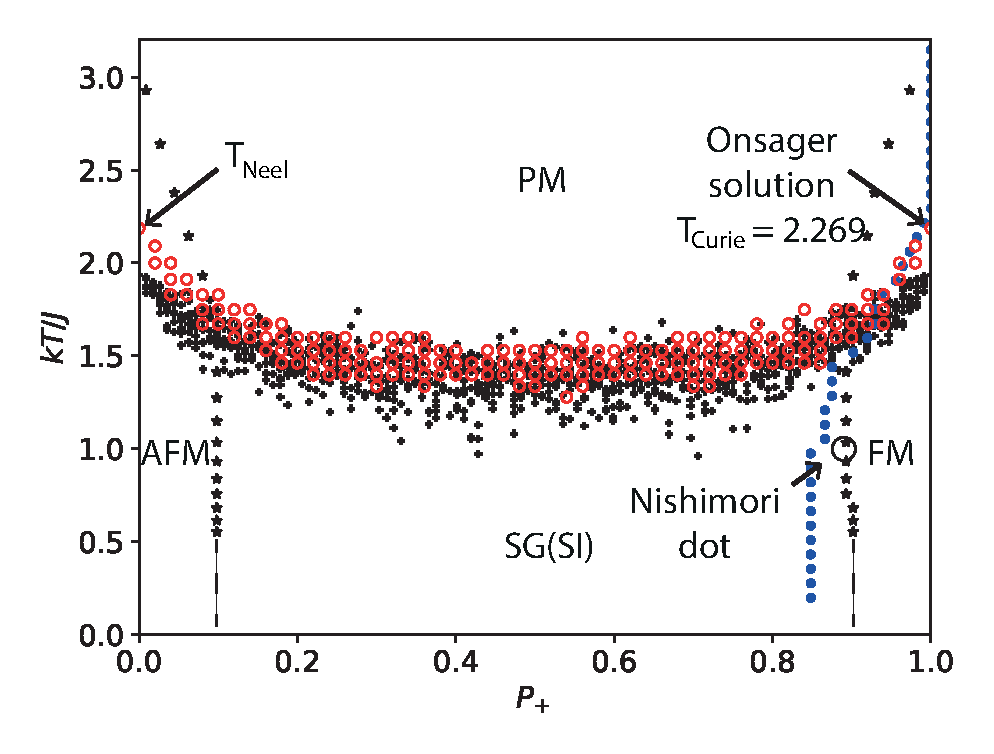
\includegraphics[width=0.8\linewidth]{Phase_diagram_h0_with_vashche_all.eps}
	\caption{Теоретическая магнитная фазовая диаграмма в отсутствии внешнего магнитного поля. Черные крестики --- точный расчет температуры максимума теплоемкости, красные пустые кружочки --- температура максимума теплоемкости, рассчитанная методом Метрополиса, синие заполненные кружочки ---  рассчитанные значения модуля намагниченности, звездочки --- результаты получены по перегибу параметра порядка.}
	\label{fig:Diag}
\end{figure}

Круглые точки получены следующим образом: считалась вероятность ферромагнетизма по заданному значению модуля спинового избытка (\ref{eq:P_M}) при определенной температуре, затем находилась конфигурация, при которой вероятность ферромагнетизма $P(FM)$ становится меньше $0.95$ и ставилась точка на график (рис. \ref{fig:Diag}).

\begin{equation}
	P(E_{gs}) =\frac{g_{gs}}{Z} \exp\left\{-\frac{E_{gs}}{kT}\right\},
	\label{eq:P_M}
\end{equation}
при этом для спинового избытка основного состояния $M_{gs}$ выполнялось неравенство

\begin{equation}
	\frac{|M_{gs}|}{N} > 0.95.
	\label{eq:M/N}
\end{equation}

$|M_{gs}|$ берется из набора основных состояний максимального значения спинового избытка, поскольку это наиболее сильно характеризует его как ферромагнетик.

На рисунке \ref{fig:Diag} красными пустыми кружками представлены результаты вычисления температуры максимума теплоемкости методом Метрополиса для систем $N=40\times40$  \cite{Metropolis53}. Стоит отметить, что рассчитанная методом Монте-Карло температура Кюри $T_{c}=2.187$ в ферромагнитной модели находится очень близко с точным решением $T_{Curie}=2.269$, которое было получено Онсагером, например, в работе \cite{Zaiman1953}. Другим важным подтверждением достоверности и данных с помощью Монте-Карло, и полученных строгим расчетом представленных данных, можно считать явление эффекта числа частиц, которое влияет на рост температуры фазового перехода для ферромагнетика (антиферромагнетика). Эти же температура и среднее значение обменной константы находятся в согласии с данными численного расчета точки перегиба параметра фрустраций, который отражает температурную зависимость роста количества возбуждений в системе взаимодействующих спинов. Более низкие значения критических температур для $P_+$ для меньших $N$ обусловлены наличием эффекта конечного размера. Так же граница ферромагнетик-спиновое стекло совпадает с приводимой в работах \cite{Hasenbusch2008, nishimori1980exact} точкой Нишимори.

В отсутствии внешнего магнитного поля при концентрации $P_{+}>0.89$ при $T \rightarrow0$ конфигурации основных состояний исследуемых численно образцов будут иметь отличный от нуля модуль спинового избытка. При этом часть конфигураций будет иметь положительный спиновый избыток, а другая часть будет иметь точно такой же по значению, но отрицательный. Наблюдается симметрия значений. При бесконечном времени ожидания и при отличных от нуля температурах система должна побывать во всех состояниях (что является главным условием термодинамического равновесия), поэтому средний по конфигурациям магнитный момент должен быть равен нулю. 

\begin{figure}[!ht]
	\centering
	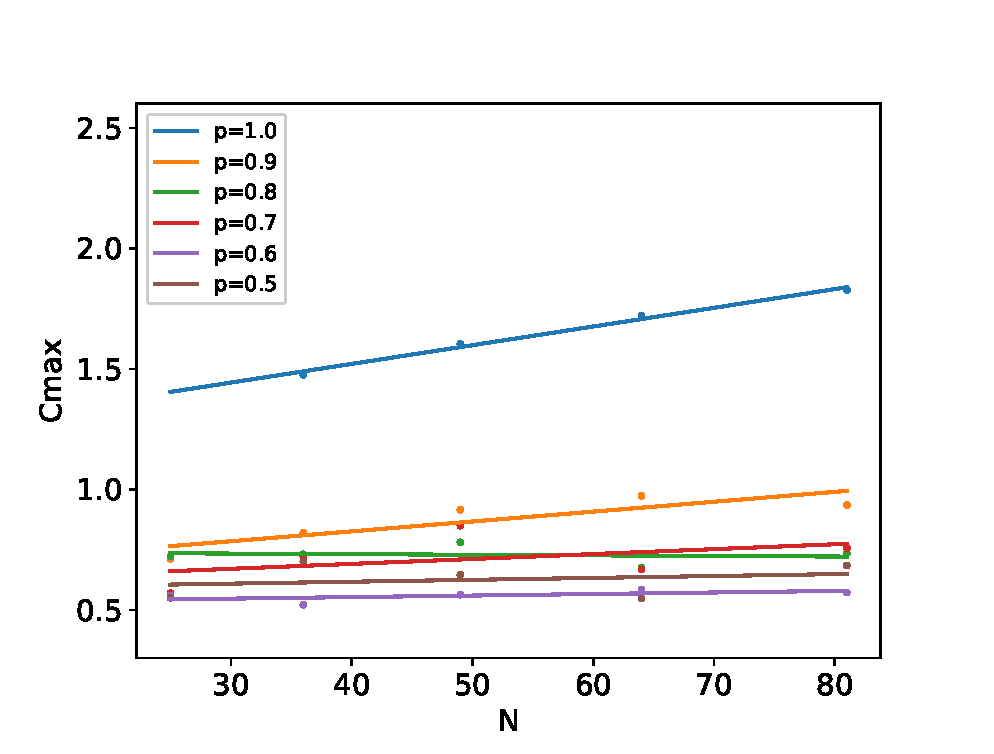
\includegraphics[width=0.8\linewidth]{Cmax(N)_scaling.eps}
	\caption{Расходимость теплоемкости в зависимости от количества  $N$ взаимодействующих спинов. На вкладке показаны значения $P_+$.}
	\label{fig:Cmax(N)_scaling}
\end{figure}

На рисунке \ref{fig:Cmax(N)_scaling} приводится зависимость максимального значения теплоемкости при критической температуре для различного количества $N$ взаимодействующих спинов. Наблюдаемый для $P_+>0.89$ рост максимального значения в поведении теплоемкости при критической температуре обычно называют расходимостью или сингулярностью. В данном случае при $P_+>0.89$ наличие расходимости в поведении теплоемкости системы взаимодействующих спинов обусловлено существованием фазового перехода второго рода. 

Отсутствие расходимости теплоемкости в интервале от $P_+>0.11$ до $P_+>0.89$ свидетельствует о существовании кроссовера, или конечной высоты пика в теплоемкости между фазой спинового стекла и фазой парамагнетика. Отсутствие сингулярности в поведении теплоемкости при переходе в фазу спинового стекла возможно связано с устройством статистической суммы, т.е пространством состояний, а именно с макроскопическим вырождением основного состояния для спиновых стекол. Для фрустрированных систем, к которым относятся спиновые стекла, существует макроскопическое вырождение основных состояний. Известно, что энтропия это своего рода ''скрытая теплота''. Поэтому при переходе в фазу спинового стекла при понижении температуры до критического значения уменьшение кинетической энергии движения спинов (уменьшение энергии термодинамических флуктуаций) не сопровождается ростом потенциальной энергии, которая упрочняет связи между спинами, как это имеет место в ферро- и антиферромагнетиках, а расходуется на образование возбуждений, или фрустраций. Для фрустрированных систем возбуждения сохраняются и в основных состояниях. 


При $P_+=0.0$ в антиферромагнетике и при $P_+=1.0$ в ферромагнетике существует только два основных состояния, фрустрации или возбуждения в которых отсутствуют. Например, для ферромагнетика при $T=0.0$ реализуется с одинаковой вероятностью состояние ''все спины --- вверх'', или состояние ''все спины --- вниз'', поэтому переход в эти основные состояния при понижении температуры приводит к резкому понижению свободной энергии, за счет резкого понижения энтропии (вырождения). Для конечных систем скачек изменения свободной энергии при переходе к основным состояниям будет не сильно выражен из-за больших значений вероятностей других состояний, поэтому и значения максимума в температурном поведении теплоемкости являются конечными. 


%Кроме того переход из состояний с отрицательным спиновым избытком к состоянию с положительным сопровождается преодолением потенциального барьера, что также требует увеличения времени наблюдения, которое растёт экспоненциально при уменьшении температуры, или при увеличении магнитного момента. Температура блокирования магнитного момента ''суперпарамагнитного кластера'' будет зависеть от объёма кластера, энергии анизотропии \cite{cullity2011, lubutin1997}. В реальных же системах, в том числе и в атомных кластерах, всегда существует, на ряду с энергией спин-спинового взаимодействия, энергия спин-орбитального взаимодействия, которая увеличивает потенциальный барьер, что приводит к отличной от нуля температуре, при которой может наблюдаться отличный от нуля ''заблокированный'' магнитный момент кластера \cite{lubutin1997, dietl2014, dmitriev2016}. В приведенных нами теоретических результатах температура имеет размерность обменных интегралов $J$.

%\textbf{Обнаружение системы ''суперпарамагнитного'' атомного кластера в одном из $2^{n-1}$ состоянии с отличном от нуля полным моментом возможно при уменьшении времени наблюдения системы, т.е. обнаружить систему в ферромагнитном состоянии.\cite{}}



\section{Перколяционные пороги и основное состояние}
В работе \cite{belokon2006} была приведена теоретическая магнитная фазовая диаграмма в осях критическая температура-концентрация ферромагнетика, где было показано, что согласуется с результатами \cite{newman2000efficient, jacobsen2014high, jacobsen2015critical}, что порог протекания по узлам квадратной решетки находится в пределах 0.591-0.593.

В настоящей работе представлена диаграмма $T(P_+)$, т.е. критические температуры для относительного количества ферромагнитных связей. Подтверждением достоверности теоретических оценок является, например, наблюдаемая при этом  расходимость температурного поведения теплоёмкости в области критической температуры в зависимости от числа спинов в системе. Точка наступления ферромагнетизма (антиферромагнетизма) легко обнаруживается по росту значения максимума теплоемкости для образцов различного $N$. Наши теоретические данные также согласуются с другими расчетами, см. например, точку Нишимори \cite{nishimori1980exact}, рисунок \ref{fig:Diag}. 

\begin{figure}[!ht]
	\centering
	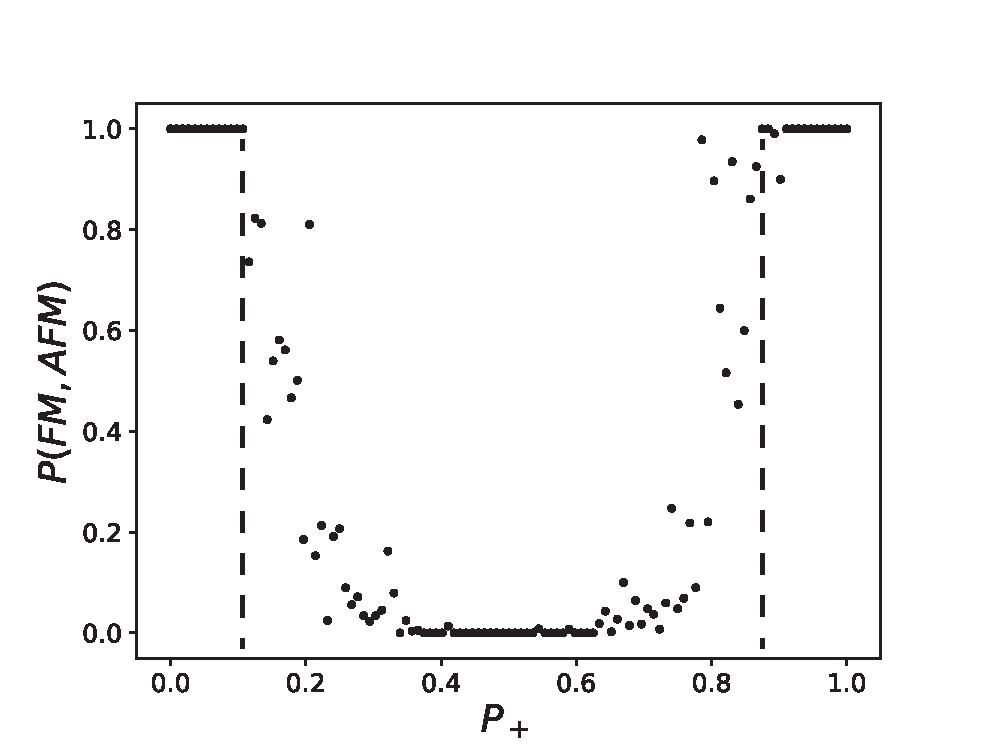
\includegraphics[width=0.8\linewidth]{Percolation.eps}
	\caption{Вероятность реализации перколяционного кластера спинов в основном состоянии, т.е. вероятность ферромагнетизма (антиферромагнетизма)}
	\label{fig:Percolation}
\end{figure}

Дополнительным теоретическим методом разделения фаз ферромагнетизма (антиферромагнетизма) и спинового стекла послужили численные расчеты перколяции спиновых кластеров, находящихся в основном состоянии. Для всех возможных конфигурации основного состояния каждого образца с фиксированным распределением обменных констант был произведен численный расчет. Вероятность появления кластера спинов основного состоянии такого, что он соединяет противоположные стороны образца, т.е. относительное число конфигураций основного состояния с наличием перколяции, в зависимости от распределения обменных констант, представлена на рисунке $\ref{fig:Percolation}$.  

Это позволяет легко различить фазы антиферромагнетизма и ферромагнетизма, наступающие при $H \rightarrow 0$ и $T \rightarrow 0$. Существует область концентрации $0.11<P_{+}<0.88$, характерной для спинового стекла, для которой у всех численно исследованных образцов наблюдаются мелкодисперсные кластеры в конфигурациях основного состояния, перколяционный кластер отсутствует.

\section{Фазовые переходы и кроссоверы в отличном от нуля внешнем магнитном поле.}

Строгое решение позволило построить теоретические магнитные фазовые диаграммы для плоской модели Изинга в отличном от нуля внешнем магнитном поле $T(P_{+},H)$. На рисунке \ref{fig:Diag1} представлена теоретическая магнитная фазовая диаграмма в магнитном поле $H=1.0$ в единицах $J$. Можно видеть наличие областей на фазовой диаграмме, в которых возможны переходы ''парамагнетик-спиновое стекло-ферромагнетик (ферромагнетик с наведенной намагниченностью)''  и ''парамагнетик-спиновое стекло-антиферромагнетик''. При этом на рисунке \ref{fig:Diag1} видно, что антиферромагнетик существует для $H=1.0$, что подтверждает не только расчет параметра фрустраций, но и температура Нееля, которая остается такой же, как при отсутствии внешнего магнитного поля.


\begin{figure}[!ht]
	\centering
	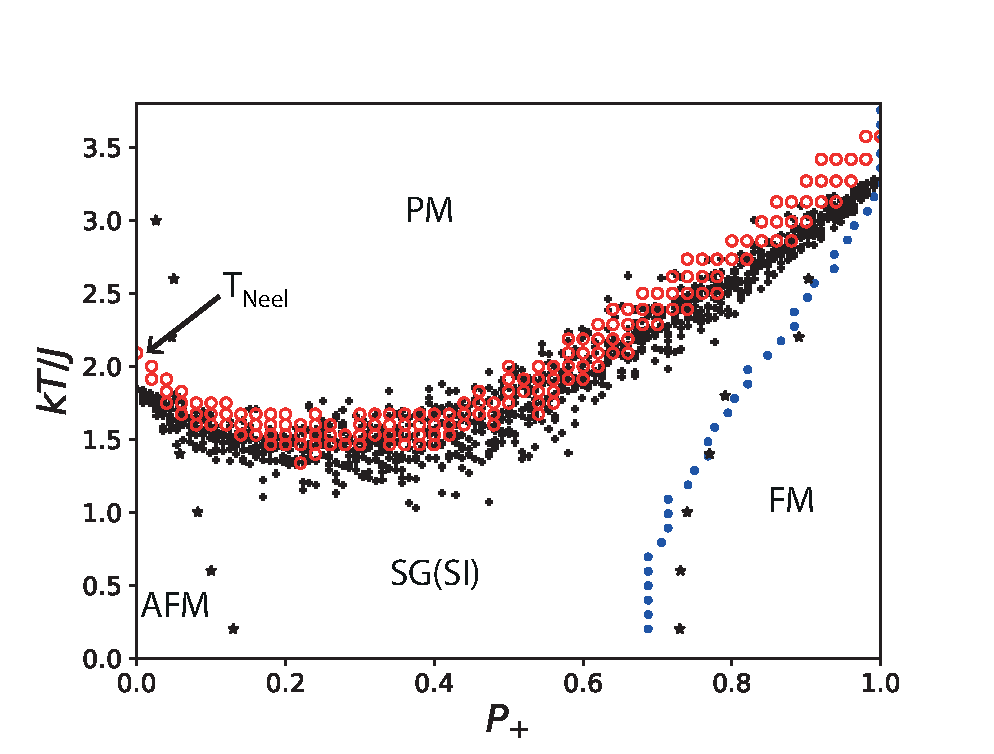
\includegraphics[width=0.8\linewidth]{Phase_diagram1_h1.0.eps}
	\caption{Фазовая диаграмма модели Изинга в поле $H = 1.0$.}
	\label{fig:Diag1}
\end{figure}

\begin{figure}[!ht]
	\centering
	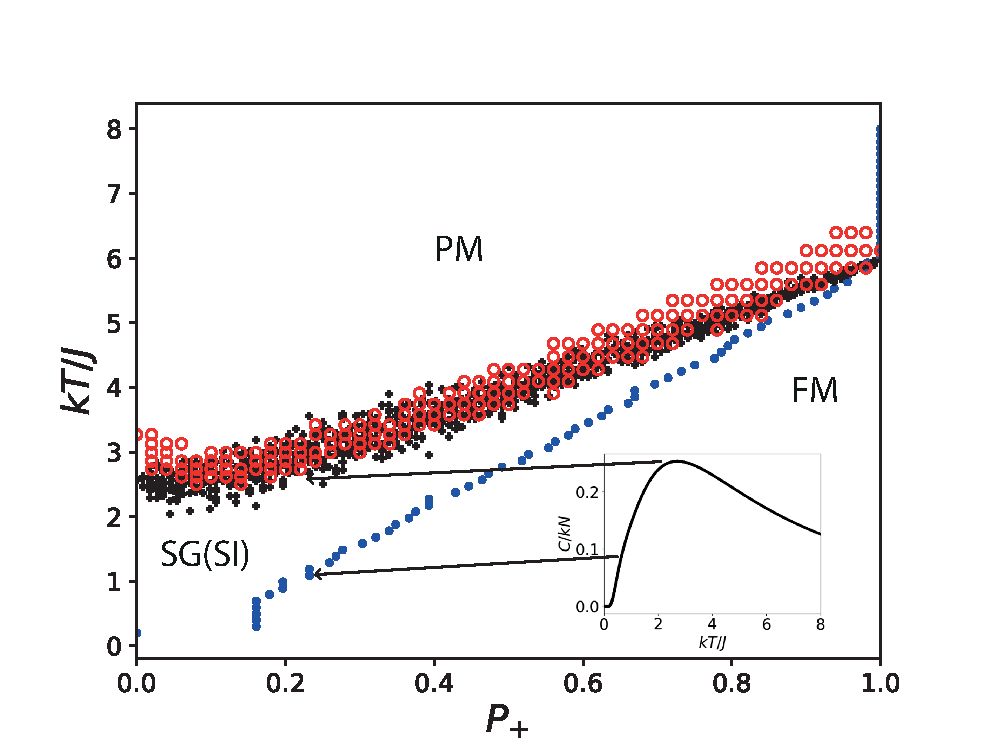
\includegraphics[width=0.8\linewidth]{Phase_diagram1_h4.0.eps}
	\caption{Фазовая диаграмма образцов в поле $H = 4.0$. На вкладке представлено температурное поведение теплоемкости $P_{+}=0.25$.}
	\label{fig:Diag4}
\end{figure}

Фазовая диаграмма в отличном от нуля относительно большом магнитном поле $H=4$ в единицах $J$ (рис. \ref{fig:Diag4}) позволяет заключить, что при увеличении модуля напряженности внешнего магнитного поля фаза антиферромагнетика подавляется полем. При этом состояние спинового стекла не исчезает бесследно. Расширяется область концентраций, для которой имеют место переходы ''парамагнетик-спиновое стекло-ферромагнетик''. В больших магнитных полях ошибка определения точки перегиба параметра фрустраций не позволяет использовать его для определения границы ферромагнитной фазы.  

Более высокая температура максимума теплоемкости для антиферромагнитной модели во внешнем магнитном поле по сравнению с $T_{Neel}$ свидетельствует о том, что произошло опрокидывание антиферромагнетика. На вкладке мы представили температурное поведение теплоемкости во внешнем магнитном поле для $P_+=0.25$. Никакой особенности теплоемкость не испытывает при переходе к возникновению наведенного ферромагнетизма.